\documentclass[xcolor=table,aspectratio=169]{beamer}
\usepackage{beamerthemesplit}
\usepackage{wrapfig}
\usetheme{SPbGU}
\usepackage{pdfpages}
\usepackage{amsmath}
\usepackage{cmap} 
\usepackage[T2A]{fontenc} 
\usepackage[utf8]{inputenc}
\usepackage[english,russian]{babel}
\usepackage{indentfirst}
\usepackage{tikz}
\usepackage{multirow}
\usepackage[noend]{algpseudocode}
\usepackage{algorithm}
\usepackage{algorithmicx}
\usetikzlibrary{shapes,arrows}
%usepackage{fancyvrb}
%\usepackage{minted}
%\usepackage{verbments}


\newtheorem{rutheorem}{Теорема}
\newtheorem{ruproof}{Доказательство}
\newtheorem{rudefinition}{Определение}
\newtheorem{rulemma}{Лемма}
\beamertemplatenavigationsymbolsempty

\title[CFPQ]{Formal Languages Theory is Not Only a Parsing}
%\subtitle[YaccConstructor]{Parsing techniques for graph analysis}
% То, что в квадратных скобках, отображается в левом нижнем углу. 
\institute[JetBrains Research]{
JetBrains Research, Programming Languages and Tools Lab
}

% То, что в квадратных скобках, отображается в левом нижнем углу.
\author[Semyon Grigorev]{Semyon Grigorev}

\date{13.04.2018}

\definecolor{orange}{RGB}{179,36,31}

\begin{document}
{
\begin{frame}[fragile]
   \begin{center}
      
\includegraphics[height=1.5cm]{pictures/JBLogo3.pdf}
    \end{center}
  \titlepage
\end{frame}
}

\begin{frame}[fragile]
  \transwipe[direction=90]
  \frametitle{Paths in graphs}
  \begin{itemize}
  \item Graph analysis
    \begin{itemize}
        \item Graph database querying
        \item Network analysis (social networks, Internet, etc)
    \end{itemize}
  \item Static code analysis
      \begin{itemize}
        \item Alias analysis
        \item Taint analysis
        \item Types-related problems
        \item Static analysis of string-embedded languages
      \end{itemize}
   \item ...
  \end{itemize}
\end{frame}

\begin{frame}[fragile]
  \transwipe[direction=90]
  \frametitle{Language constrained path querying}
  Language-constrained path querying, language reachability
  \begin{itemize}
  \item $\Sigma$ is a set of terminals 
  \item $L(\Sigma)$ is a language over $\Sigma$
  \item $G = (V,E,D)$ is a directed graph, $E \subseteq V\times D \times V$, $D\subseteq \Sigma$
  \item $p = v_0 \xrightarrow{l_0} v_1 \xrightarrow{l_1} \cdots v_{n-1}\xrightarrow{l_{n-1}}v_n$ is a path in $G$
  \item $w(p) = w(v_0 \xrightarrow{l_0} v_1 \xrightarrow{l_1} \cdots v_{n-1}\xrightarrow{l_{n-1}}v_n) = l_0 l_1 \cdots l_{n-1}$
  \item $R =\{ p \ | \ w(p) \in L(\Sigma)\}$
  \begin{itemize}
    \item \textbf{Problem:} $R$ can be an infinite in some cases
  \end{itemize}
  \item Task may be formulated in other way: $Q =\{ (v_0,v_n) \ | \ \exists p = v_0 \xrightarrow{l_0} \cdots \xrightarrow{l_{n-1}}v_n \ (w(p) \in 
  L(\Sigma))\}$
  \end{itemize}
\end{frame}


\begin{frame}[fragile]
  \transwipe[direction=90]
  \frametitle{Regular constarints}
  \begin{itemize}
  \item $L(\Sigma)$ is a regular language
    \begin{itemize}
      \item Graph databases query languages (SPARQL, Cypher, PGQL)
      \item OpenCypher: \url{https://goo.gl/5h5a8P}
    \end{itemize}  
  \end{itemize}
\end{frame}


\begin{frame}[fragile]
  \transwipe[direction=90]
  \frametitle{Context-free constraints}
  \begin{itemize}
  \item $L(\Sigma)$ is a context-free language
  \item Graph databases and semantic networks
    \begin{itemize}
        \item \emph{Sevon P., Eronen L.} ``Subgraph queries by context-free grammars.'' 2008
        \item \emph{Zhang X. et al.} ``Context-free path queries on RDF graphs.'' 2016
        \item \emph{Hellings J.} ``Conjunctive context-free path queries.'' 2014
    \end{itemize}
    \item Static code analysis
    \begin{itemize}
        \item \emph{Thomas Reps et al.} ``Precise interprocedural dataflow analysis via graph reachability.'' 1995 
        \item \emph{Qirun Zhang et al.}  ``Efficient subcubic alias analysis for C.'' 2014
        \item \emph{Dacong Yan et al.} ``Demand-driven context-sensitive alias analysis for Java.'' 2011
        \item \emph{Jakob Rehof and Manuel Fahndrich.} ``Type-base flow analysis: from polymorphic subtyping to CFL-reachability.'' 2001
    \end{itemize}
  \end{itemize}
\end{frame}


\begin{frame}
  \transwipe[direction=90]
  \frametitle{Context-free constarints}

\begin{itemize} 
\item \emph{Kai Wang et. al.} Graspan: A Single-machine Disk-based Graph System for Interprocedural 
Static Analyses of Large-scale Systems Code. 2017
  
\begin{itemize} 
   \item `` We have identified a total of 1127 unnecessary NULL tests in Linux, 149 in PostgreSQL, 
   32 in httpd.''
   \item ``Our analyses reported 108 new NULL pointer dereference bugs in Linux, among which 23 are false positives''
   \item ``For PostgreSQL and httpd, we detected 33 and 14 new NULL pointer bugs; our manual 
   validation did not find any false positives among them.''
\end{itemize}

\end{itemize}

\end{frame}

\begin{frame}
  \transwipe[direction=90]
  \frametitle{Linear-conjunctive constraints}

\begin{itemize} 
  \item $L(\Sigma)$ is a linear-conjunctive language
    \begin{itemize} 
      \item Interleaving of balcned brackets: $L_1 = \{a^n b^n | n \geq 0\}; L_2 = \{c^m d^m | m \geq 0\}; L_3 = L_1 \odot L_2 = \{a b; a c b c d d; c d a b;  \dots\}$
    \end{itemize}

  \item \emph{Qirun Zhang and Zhendong Su.} Context-sensitive data-dependence analysis via linear conjunctive language reachability. 2017
  
\end{itemize}

\end{frame}


\begin{frame}[fragile]
  \transwipe[direction=90]
  \frametitle{Chelenges}
  \begin{itemize}
  \item Theoretical open problem
    \begin{itemize}
        \item Is there exists an algorithm with time complexity $O(|V|^{3-\varepsilon}), \varepsilon > 0$
    \end{itemize}
  \item Practical utilisation of solutions from ``classical'' parsing
    \begin{itemize}
        \item Algorithms: CYK, (Generalized) LL, (Generalized) LR, Earley, ...
        \item Techniques: parser combinators, parser generators, ... 
        \item Advanced techniques: GPGPU utilzation, advanced data structures (compact parse forest representation, graph structured stack), ...
    \end{itemize}
  \item Huge amount of data requires efficien implementation of parallel and/or destributed query processing
  \end{itemize}

\end{frame}

\begin{frame}[fragile]
  \transwipe[direction=90]
  \frametitle{Our experiments}

\begin{itemize} 
\item Generalized LL for CFPQ (GLL)
\begin{itemize} 
  \item Based on Generalized LL: \emph{Scott E., Johnstone A.} ``GLL parsing''
  \item Time complexity: $O\left(|V|^3*\max\limits_{v \in V}\left(deg^+\left(v\right)\right)\right)$
  \item \emph{Semyon Grigorev and Anastasiya Ragozina.} ``Context-free path querying with structural 
  representation of result.'' 2017
\end{itemize}
\item GPGPU utilization for CFPQ (GPGPU)
\begin{itemize} 
   \item Based on \emph{Valiant L.} ``General context-free recognition in less than cubic time.'' 1974
   \item Time complexity: $O(|V|^2 |N|^3(BMM(|V|) + BMU (|V|)))$
     \begin{itemize} 
      \item $BMM(n)$ --- boolean matrix multiplcation $n\times n$
      \item $BMU(n)$ --- cell-by-cell \verb|or| $n\times n$
     \end{itemize}
   \item \emph{Rustam Azimov, Semyon Grigorev.} ``Context-Free Path Querying by Matrix 
     Multiplication.'' 2017
\end{itemize}
\item Parser-Combinators for Context-Free Path Querying (in Scala)
\end{itemize}
\end{frame}


\begin{frame}[fragile]
\transwipe[direction=90]
\frametitle{Performance comparison setup}
%\centering
\begin{figure}[ht]
%   \begin{center}
   \centering
%   \begin{subfigure}[b]{0.4\textwidth}

   \[
\begin{array}{rl}
   0: & \textbf{S} \rightarrow \text{\textit{subClassOf}}^{-1} \ \textbf{S} \ \text{\textit{subClassOf}} \\ 
   1: & \textbf{S} \rightarrow \text{\textit{type}}^{-1} \ \textbf{S} \ \text{\textit{type}} \\ 
   2: & \textbf{S} \rightarrow \text{\textit{subClassOf}}^{-1} \ \text{\textit{subClassOf}} \\ 
   3: & \textbf{S} \rightarrow \text{\textit{type}}^{-1} \ \text{\textit{type}} \\ 
\end{array}
\]
   Query 1
   \end{figure}
\begin{figure}[h]%{0.4\textwidth}
   \centering

   \[
\begin{array}{rl}
   0: & \textbf{S} \rightarrow \textbf{B} \ \text{\textit{subClassOf}} \\ 
   1: & \textbf{S} \rightarrow \text{\textit{subClassOf}} \\ 
   2: & \textbf{B} \rightarrow \text{\textit{subClassOf}}^{-1} \ \textbf{B} \ \text{\textit{subClassOf}} \\
   3: & \textbf{B} \rightarrow \text{\textit{subClassOf}}^{-1} \ \text{\textit{subClassOf}} \\ 
\end{array}
\]
   Query 2

   \end{figure}

\end{frame}


\begin{frame}[fragile]
\transwipe[direction=90]
\frametitle{Performance comparison result}
\centering
\rowcolors{1}{}{lightgray}
\begin{tabular}{  c | c | c | c | c | c | c | c }
%\hline
\textnumero & \#V & \#E & \multicolumn{3}{c|}{Query 1 (ms)} & \multicolumn{2}{c}{Query 2 (ms)} \\
\cline{4-8}
& & & CYK\footnote{Zhang, et al. ``Context-free path queries on RDF graphs.''} & GLL & GPGPU & GLL & GPGPU \\
\hline 
\hline
1  & 144  & 323   & 1044    & 10   & 12  & 1   & 1 \\
2  & 129  & 351   & 6091    & 19   & 13  & 1   & 0 \\
3  & 131  & 397   & 13971   & 24   & 30  & 1   & 10 \\
4  & 179  & 413   & 20981   & 25   & 15  & 11  & 9 \\
5  & 337  & 834   & 82081   & 89   & 32  & 3   & 6 \\
6  & 291  & 685   & 515285  & 255  & 22  & 66  & 2 \\
7  & 341  & 711   & 420604  & 261  & 20  & 45  & 24 \\
8  & 671  & 2604  & 3233587 & 697  & 24  & 29  & 23 \\
9  & 733  & 2450  & 4075319 & 819  & 54  & 8   & 6 \\
10 & 6224 & 11840 & --      & 1926 & 82  & 167 & 38\\
11 & 5864 & 19600 & --      & 6246 & 185 & 46  & 21\\
12 & 5368 & 20832 & --      & 7014 & 127 & 393 & 40\\

%\hline
\end{tabular}

\end{frame}
        
\begin{frame}
\transwipe[direction=90]
\frametitle{Info}
\begin{itemize}
  \item E-mail: \url{semen.grigorev@jetbrains.com}
  \item GitHub-community YaccConstructor: \url{https://github.com/YaccConstructor}
\end{itemize}
\end{frame}


\begin{frame}[fragile]
  \transwipe[direction=90]
  \frametitle{Example}
%\begin{figure}[ht]
Input graph 
\vspace{-0.5cm}
\begin{center}
        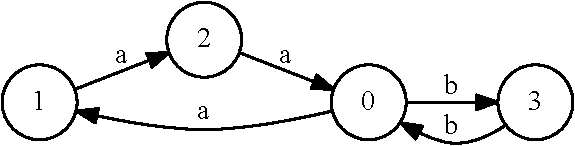
\includegraphics[height=0.2\textheight]{pictures/input.pdf} 
\end{center}
query is a grammar $G$ which specifies the language $L=\{a^n b^n \ | \ n \geq 1\}$\\
\begin{center}
   \[
\begin{array}{rl} 
   0:& S \rightarrow a \ S \ b \\
   1:& S \rightarrow Middle \\
   2:& Middle \rightarrow a \ b
\end{array}
\]
\end{center}
\vspace{0.8em}
Query result is an infinite set of paths
\begin{itemize}
\item $p_1 = 0\xrightarrow{a}1\xrightarrow{a}2\xrightarrow{a}0\xrightarrow{b}3\xrightarrow{b}0\xrightarrow{b}3$
\item $p_2 = 0\xrightarrow{a}1\xrightarrow{a}2\xrightarrow{a}0\xrightarrow{a}1\xrightarrow{a}2\xrightarrow{a}0\xrightarrow{b}3\xrightarrow{b}0\xrightarrow{b}3\xrightarrow{b}0\xrightarrow{b}3\xrightarrow{b}0$
\item ...
\end{itemize}

\end{frame}

\begin{frame}[fragile]
  \transwipe[direction=90]
  \frametitle{Structural representation of query result}
\vspace{-0.3cm}
\begin{figure}[ht]
    \centering
        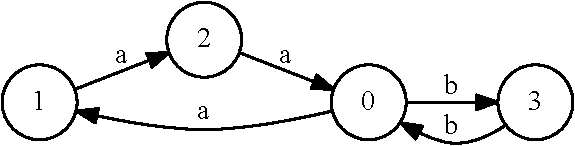
\includegraphics[width=0.45\textwidth]{pictures/input.pdf} \\
        Input graph
\end{figure}
\vspace{-0.2cm}
\begin{center}
\begin{tabular}{  c  c  c  }
      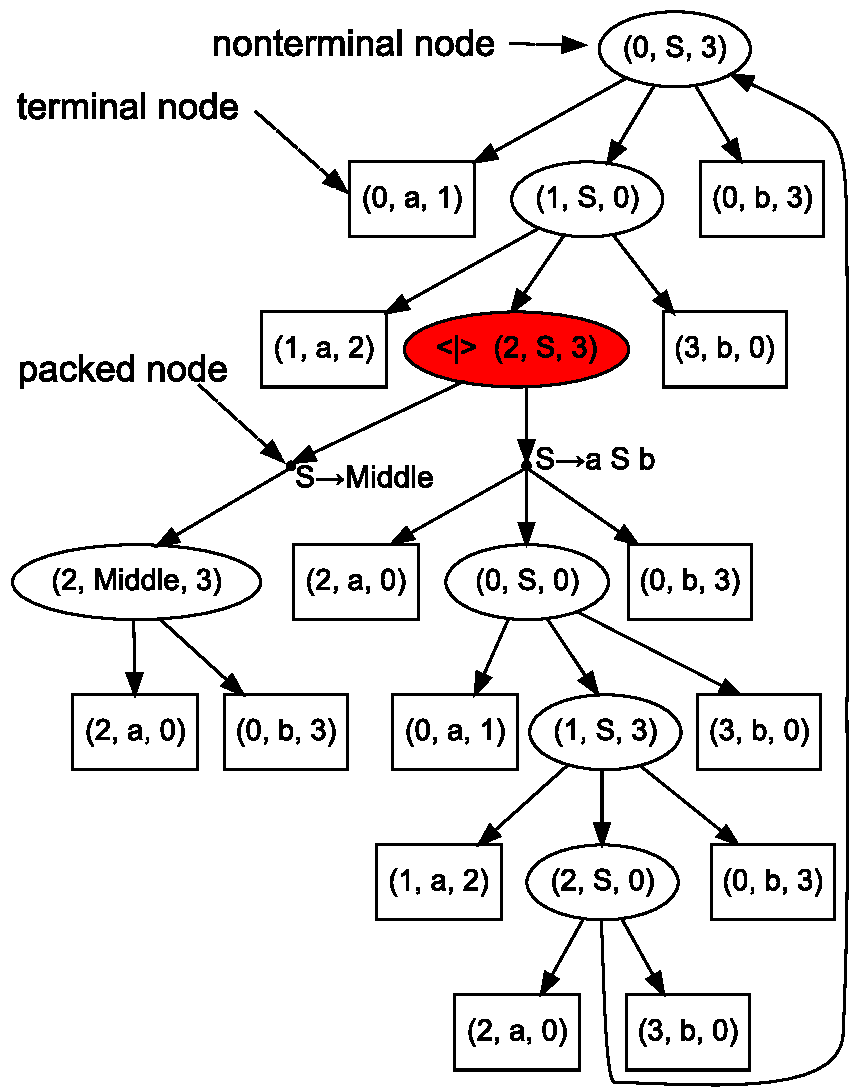
\includegraphics[height=4.5cm]{pictures/AnBn.pdf}
    &
      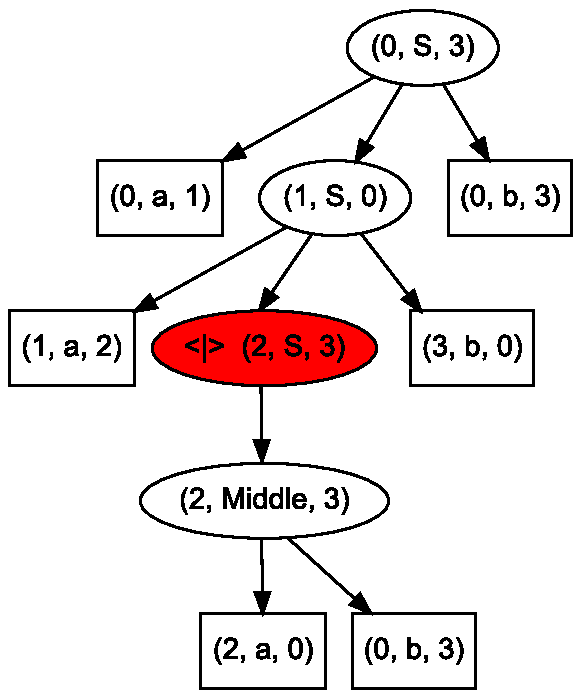
\includegraphics[height=4.5cm]{pictures/AnBn_2.pdf}
    &
      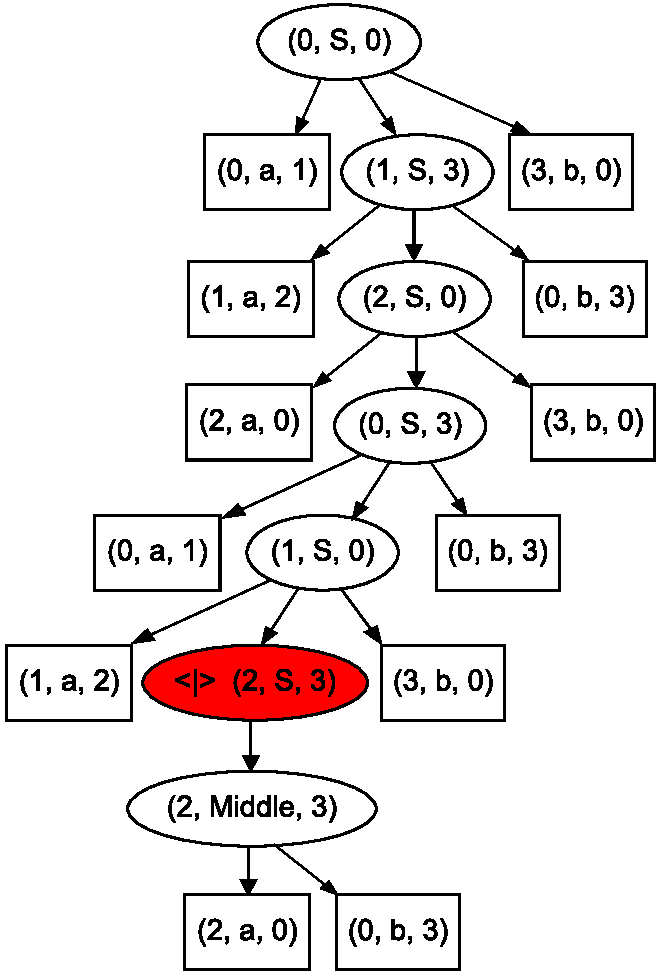
\includegraphics[height=4.5cm]{pictures/AnBn_1.pdf}

\\
\small{Query result (SPPF)}
& \small{Tree for path $p_1$}
& \small{Tree for path $p_2$}
  \end{tabular}
\end{center}                
\end{frame}

\begin{frame}[fragile]
  \transwipe[direction=90]
  \frametitle{Paths extraction}
\begin{center}

\begin{minipage}{0.4\textwidth}
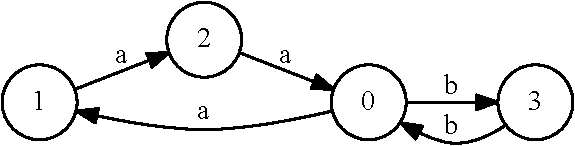
\includegraphics[width=0.9\textwidth]{pictures/input.pdf}
\\
Path: $0\xrightarrow{a}1\xrightarrow{a}2\xrightarrow{a}0\xrightarrow{b}3\xrightarrow{b}0\xrightarrow{b}3$
\end{minipage}
~
\begin{minipage} {0.57\textwidth}
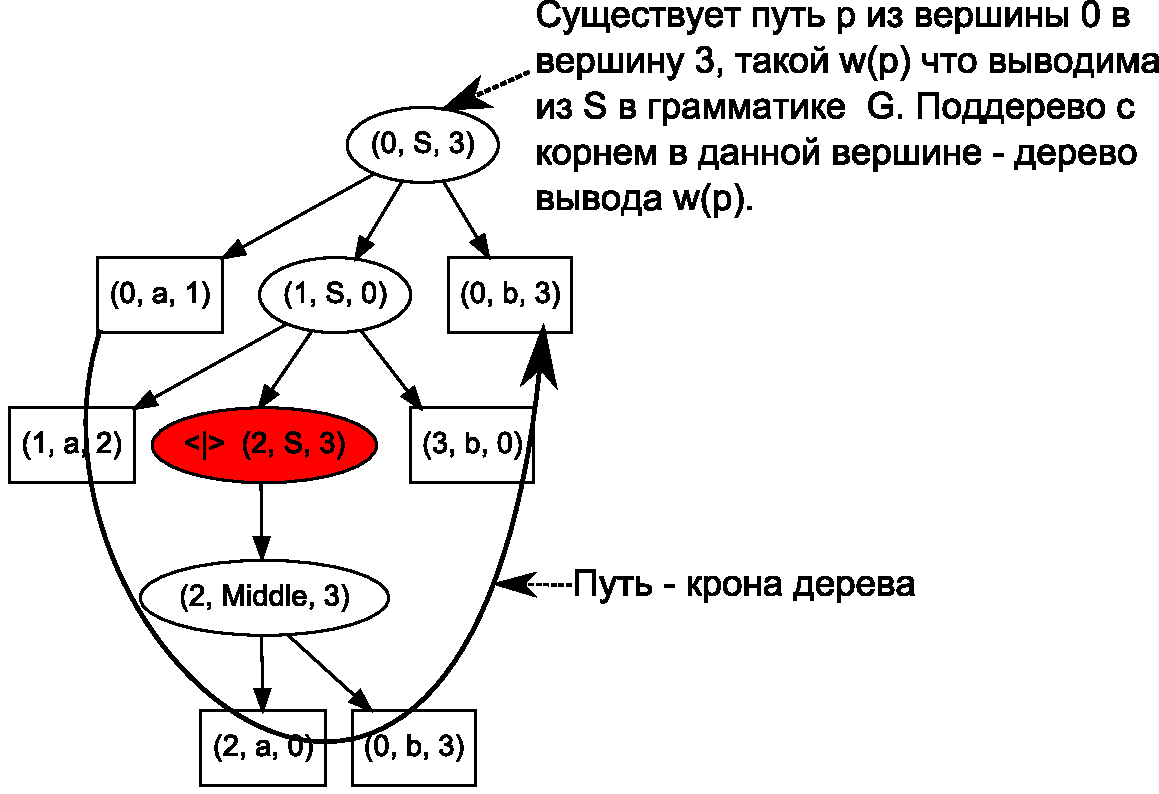
\includegraphics[width=0.99\textwidth]{pictures/AnBn_2_m.pdf}
\end{minipage}

        
\end{center}                
\end{frame}


\begin{frame}[fragile]
  \transwipe[direction=90]
  \frametitle{Key idea}
Context-free languages are closed under intersection with regular languages
\pause
\vspace{-0.2cm}
\begin{center}
\begin{tabular}{  l p{4cm} l  }
    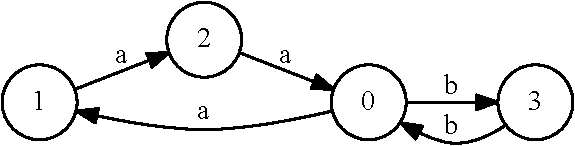
\includegraphics[width=0.35\textwidth]{pictures/input.pdf}
    & &
$
 
\begin{array}{rl} 
   0:& S \rightarrow a \ S \ b \\
   1:& S \rightarrow Middle \\
   2:& Middle \rightarrow a \ b
\end{array}

$
\end{tabular}

\vspace{-0.65cm}
\pause

\begin{tabular}{  l p{2cm}  l  }
    \raisebox{-0.5\totalheight}{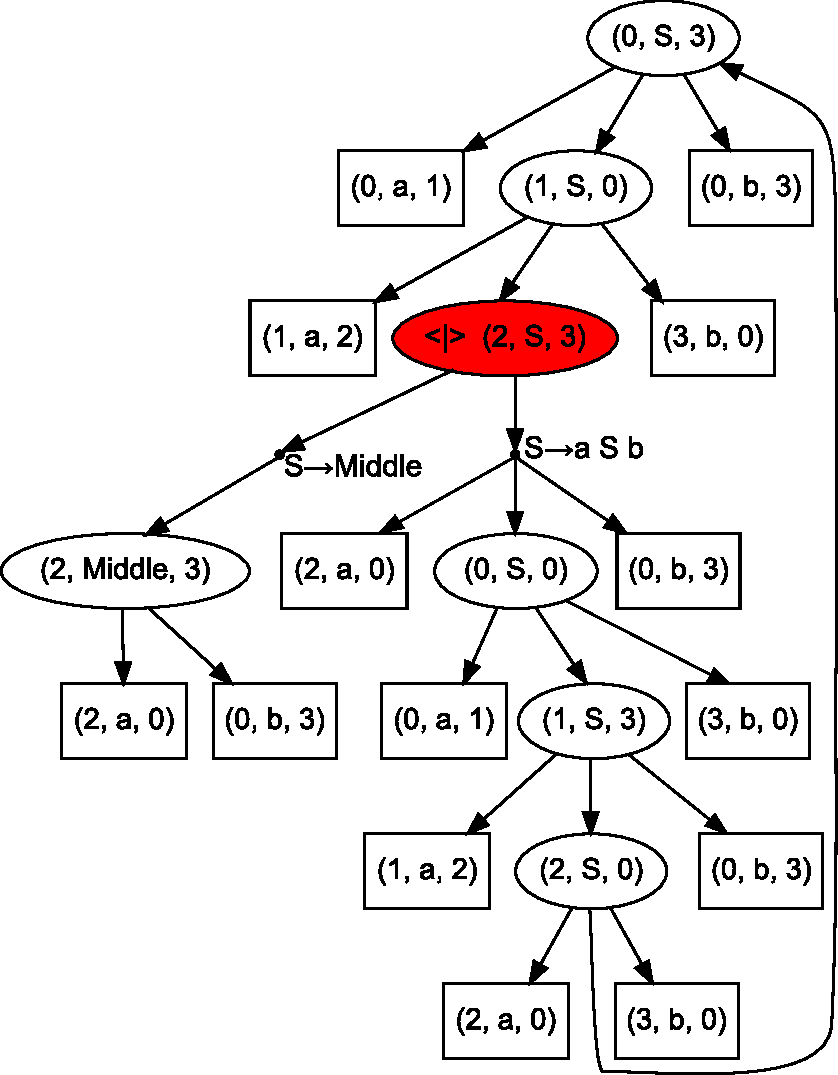
\includegraphics[width=0.29\textwidth]{pictures/AnBn_m.pdf}}
    &
    &
$
\begin{array}{rl} 
   (0,S,3) & \rightarrow (0,a,1) \ (1,S,0) \ (0,b,3) \\
   (1,S,0) & \rightarrow (1,a,2) \ (2,S,3) \ (3,b,0) \\
   (2,S,3) & \rightarrow (2,a,0) \ (0,S,0) \ (0,b,3) \\
   (2,S,3) & \rightarrow (2,Middle,3)                \\
   (0,S,0) & \rightarrow (0,a,1) \ (1,S,3) \ (3,b,0) \\
   (1,S,3) & \rightarrow (1,a,2) \ (2,S,0) \ (0,b,3) \\
   (2,S,0) & \rightarrow (2,a,0) \ (0,S,3) \ (3,b,0) \\
   (0,Middle,3) & \rightarrow (2,a,0) \ (0,b,3)  \\
\end{array}
$

\end{tabular}
\end{center}                
\end{frame}

\end{document}